\chapter{Appendix}

% \section{To the proof of the theorem of Peano}

% \begin{definition}
%   A function sequence $f^n$ is called \textbf{equicontinuous}, if it holds:
%   \begin{gather*}
%   \forall \,\epsilon > 0
%   \;\exists \, \delta > 0
%   \;\forall \, n \in \mathbb{N}
%   \;\forall |y-x| < \delta 
%   \quad:\quad |f^n(y)-f^n(x)| < \epsilon    
%   \end{gather*}
% \end{definition}

% \begin{theorem}[Arzela-Ascoli]\label{theorem:arzelaascoli}
%   Let be $f^h$ a equicontinuous, uniformly bounded sequence
%   of functions. Then it exists a subsequence $f^{h_i}$ which converges to a 
% 	uniformly continuous function $f$.
% \end{theorem}

% \begin{todo}
% \begin{proof}
%   Nachzulesen in ...? %%%%%%%%%%%%%%%%
% \end{proof}
% \end{todo}

% \begin{proof}[Proof of the theorem of Peano]
%   I) Choose a sequence $h \to 0$ and compute approximations $u^h(t)$ with  
% 		Euler's method.

%     The method is well-defined, 
% 		if $(t_n,u_n^h) \in D \ \ \ \forall n$ with $|t_n-t_0| \le T$

%     $|u_1^h - u_0| = |h f(t_0,u_0)| \le h M$

%     $|u_n^h - u_0| = | \sum\limits_{k=0}^{n-1} h f(t_k,u_k^h) | 
% 		\le M \underbrace{h n}_{= T} \le M T \le \beta$

%   \noindent II) To show: $u^h(t)$ is uniformly bounded and 
% 		equicontinuous.

%     a) Since $u^h(t) \in D \Rightarrow |u^h(t)-u_0| \le \beta$

%     b) For $\tau,t \in [t_{n-1},t_n]$ holds $|u^h(\tau)-u^h(t)| \le M |\tau-t|$

%     \noindent $\Rightarrow$ The functions $u^h$ are equicontinuous and 
% 		Lipschitz continuous with L-constant $M$.

%     \noindent $\underset{Theorem~\ref{Theorem:arzelaascoli} }{\Rightarrow}$ It exists
% 		a sequence $u_i^h$ with $u_i^h \to u$ and $u$ is equicontinuous.

%   \noindent III) The limit function $u$ solves Volterra's integral equation

%     $u(t) = u_0 + \int\limits_{t_0}^t f(s,u(s))\ \mathrm{d}s$.

%     \noindent To that: (The subsequence index will be omitted in the following)

%     $u^h(t) = u_0 + \sum\limits_{j=0}^k h f(t_j,u_j^h) + (t-t_k) f(t_k,u_k^h)$,

%     \noindent where $t_k$ is the highest point of Euler's method with $t_k < t$.

%     $\begin{array}{lcl}
%       u^h(t) = u_0 + \int\limits_{t_0}^t \Phi^h(s) \ \mathrm{d}s
%         & \text{ with } & \Phi^h(t) = f(t_j,u_j^h) \text{ for } t \in [t_j,t_{j+1}]\\
%       \Big\downarrow h \to 0 & \ & \Big\downarrow h \to 0 \\
%       u(t) = u_0 + \int\limits_{t_0}^t \Phi(s) \ \mathrm{d}s
%         & \text{ with } & \Phi(t) = f(t,u(t))\\
%     \end{array}$

%     \noindent Remains to show: $\Phi^h \to \Phi$ uniformly

% 		This follows from the uniformly continuity of $f$ in $\overline{D}$ and 
% 		the equicontinuity of $u^h \to u$.
% \end{proof}

%%%%%%%%%%%%%%%%%%%%%%%%%%%%%%%%%%%%%%%%%%%%%%%%%%%%%%%%%%%%%%%%%%%%%%
%%%%%%%%%%%%%%%%%%%%%%%%%%%%%%%%%%%%%%%%%%%%%%%%%%%%%%%%%%%%%%%%%%%%%%
\section{Comments on uniqueness of an IVP}
%%%%%%%%%%%%%%%%%%%%%%%%%%%%%%%%%%%%%%%%%%%%%%%%%%%%%%%%%%%%%%%%%%%%%%
%%%%%%%%%%%%%%%%%%%%%%%%%%%%%%%%%%%%%%%%%%%%%%%%%%%%%%%%%%%%%%%%%%%%%%

	For a first order differential equation Lipschitz continuity is only a
	sufficient and not, as one might think, a necessary condition for
	uniqueness of a first order differential equation. The following theorem
	and proof show that it is indeed possible to have uniqueness of solution
	without assuming Lipschitz continuity on the function.

\begin{Theorem*}{nonnecessity}{Non-necessity of L-continuity}
	Let $f$ be a continous function satisfying $f(x) > 0$ for all
	$x \in \R$. Then, the solution to the IVP
	\begin{subequations} \label{eq:myivp}
		\begin{align}
		  u'(t)&=f\bigl(t,u(t)\bigr) \\
		  u(t_0)&=u_0
		\end{align}
	\end{subequations}
	is globally unique for all $(t_0, u_0) \in \R^2$.
\end{Theorem*}

\begin{proof}
	Assume two solutions $\varphi, \, \psi \colon I \to \R$ on an open
	intervall $I$ with $t_0 \in I$. Then, there holds
\begin{xalignat}{3}
      && 1 = \frac{\varphi(t) '}{f(\varphi(t))} = \frac{\psi(t) '}{f(\psi(t))} 
	  && \text{for all } t \in I. \label{eq:myivp2}
\end{xalignat}
	Define the function $F \colon \R \to \R$ through
\begin{gather*}
		F(x) = \int_{u_0} ^x \frac{\ds}{f(s)}.
\end{gather*}
	$F$ is continously differentiable since
\begin{gather*}
		\partial_x F(x) 
		= \partial_x \left( \int_{u_0} ^x \frac{\ds}{f(s)} \right) 
		= \frac{1}{f(x)}.
\end{gather*}
	Obviously, $F$ is also stricly increasing, hence injective on
	$\R$: Take $x, \, y \in \R$ and assume without loss of generality
	 that $x < y$. Then we have $F(x) < F(y)$ and thus $F(x) \neq F(y)$.
	 Thus, $F$ is an injection.
	
	Also, for all $t \in I$ there holds
\begin{gather*}
		F(\varphi(t))
		= \int_{u_0} ^t \frac{\varphi'(s)}{f(\varphi(s))} \ds
		\overset{\ref{eq:myivp2}}{=} \int_{u_0} ^t \frac{\psi'(s)}{f(\psi(s))} \ds
		= F(\psi(t)). 
\end{gather*}
	Thus, since $F$ is injective, we have $\varphi(t) = \psi(t)$ for all
	$t \in I$. In conclusion, the IVP \ref{eq:myivp} has a unique solution.
\end{proof}


%%%%%%%%%%%%%%%%%%%%%%%%%%%%%%%%%%%%%%%%%%%%%%%%%%%%%%%%%%%%%%%%%%%%%%
%%%%%%%%%%%%%%%%%%%%%%%%%%%%%%%%%%%%%%%%%%%%%%%%%%%%%%%%%%%%%%%%%%%%%%
\section{Properties of matrices}
%%%%%%%%%%%%%%%%%%%%%%%%%%%%%%%%%%%%%%%%%%%%%%%%%%%%%%%%%%%%%%%%%%%%%%
%%%%%%%%%%%%%%%%%%%%%%%%%%%%%%%%%%%%%%%%%%%%%%%%%%%%%%%%%%%%%%%%%%%%%%

\subsection{The matrix exponential}
\label{sec:matrix-exponentials}

\begin{definition}
  The matrix exponential $e^A$ of a matrix $A\in \R^{d\times d}$ is defined
  by its power series
  \begin{gather}
    \label{eq:appendix:1}
    e^A = \sum_{k=0}^\infty \frac{A^k}{k!}.
  \end{gather}
\end{definition}

\begin{lemma}
  \label{lemma:appendix:exp-0}
  The power series~\eqref{eq:appendix:1} converges for each matrix $A$.
\end{lemma}
\begin{proof}
  
\end{proof}

\begin{lemma}[Properties of the matrix exponential function] 
  \label{Lemma:appendix:exp-1}
	The following relations hold true:
  \begin{xalignat}2
    \label{eq:appendix:2}
    e^0 &= \identity \\
    \label{eq:appendix:3}
    e^{\alpha A} e^{\beta A} &= e^{(\alpha+\beta) A}, &\forall
    A\in\R^{d\times d}\; \forall \alpha,\beta\in \R,\\
    \label{eq:appendix:4}
    e^A e^{-A} &= \identity &\forall A\in\R^{d\times d}.
  \end{xalignat}
  Moreover, $e^A$ is invertible for arbitrary quadratic matrices $A$.
\end{lemma}

%%%%%%%%%%%%%%%%%%%%%%%%%%%%%%%%%%%%%%%%%%%%%%%%%%%%%%%%%%%%%%%%%%%%%%
%%%%%%%%%%%%%%%%%%%%%%%%%%%%%%%%%%%%%%%%%%%%%%%%%%%%%%%%%%%%%%%%%%%%%%
\section{The Banach fixed-point theorem}
%%%%%%%%%%%%%%%%%%%%%%%%%%%%%%%%%%%%%%%%%%%%%%%%%%%%%%%%%%%%%%%%%%%%%%
%%%%%%%%%%%%%%%%%%%%%%%%%%%%%%%%%%%%%%%%%%%%%%%%%%%%%%%%%%%%%%%%%%%%%%

\begin{Theorem*}{banach}{Banach fixed-point theorem}
	Let $\Omega \subset \R$ be a closed set and $f \colon \Omega \to \Omega$
	a contraction, i.e. there holds $|f(x) - f(y)| \le \gamma |x-y|$ for a
	$\gamma \in (0,1)$.

	Then there exists a unique $x^* \in \Omega$ such that $f(x^*) =x^*$.
\end{Theorem*}

\begin{proof}
	Let $x_0 \in \Omega$ and define $f(x_k) = x_{k+1}$. First, we prove
	existence unsing the cauchy-criterion. Let $k, n \in \mathbb N_0$ and consider
	\begin{gather*}
	|x_k - x_{k+m} | = |f(x_{k-1}) - f(x_{k+m-1})| \le \gamma |x_{k-1} - x_{k+m-1})|.
	\end{gather*}

	Iteratively, we get
	\begin{gather*}
	|x_k - x_{k+m} | \le \gamma^k |x_0 - x_m|.
	\end{gather*}

	We now write $x_0 - x_m = x_0 - x_1 + x_1 - x_2 + \dots + x_{m-1} - x_m$.
	The triangle-inequality yields the estimate
	\begin{gather*}
	\gamma^k |x_0 - x_m| \le \gamma^k |x_0 - x_1| + |x_1 - x_2| + \dots + |x_{m-1} - x_m|  \\
	\le \gamma^k |x_0 - x_1| (1 + \gamma + \gamma ^2 + \dots + \gamma^m) \\
	\le \frac{\gamma^k}{1-\gamma} |x_0 - x_1|.
	\end{gather*}
	As $k$ gets larger the estimate goes to zero.

	Concerning uniqueness, let $x^*$ and $y^*$ be fixpoints.
	\begin{gather*}
	|x^* - y^*| = |f(x*) - f(y^*) | \le \gamma |x^* - y^*|
	\end{gather*}
	Since $\gamma \in (0,1)$ we immediately obtain $|x^* - y^*| = 0$. Using
	that $|a| = 0$ if and only if $a=0$ yields $y^* = x^*$. This concludes the proof.
\end{proof}

%%%%%%%%%%%%%%%%%%%%%%%%%%%%%%%%%%%%%%%%%%%%%%%%%%%%%%%%%%%%%%%%%%%%%%
%%%%%%%%%%%%%%%%%%%%%%%%%%%%%%%%%%%%%%%%%%%%%%%%%%%%%%%%%%%%%%%%%%%%%%
\section{The implicit and explicit Euler-method}
%%%%%%%%%%%%%%%%%%%%%%%%%%%%%%%%%%%%%%%%%%%%%%%%%%%%%%%%%%%%%%%%%%%%%%
%%%%%%%%%%%%%%%%%%%%%%%%%%%%%%%%%%%%%%%%%%%%%%%%%%%%%%%%%%%%%%%%%%%%%%

	The explicit resp. implicit Euler is given by the one-step method
	\begin{align*}
	&& y_1 = y_0 + h f(y_0) && \text{resp.} && y_1 = y_0 + h f(y_1) &&
	\end{align*}
	Clearly, the explicit Euler is rather easy to compute since all one
	needs are $f$, $h$ and $y_0$. On the other hand, the implicit Euler
	is more difficult since for calculating $y_1$ we need the value of $f$ at $y_1$.

	Consider the following visualizations.
	\begin{center}
	\begin{minipage}[t]{0.42\textwidth}
	\begin{tikzpicture}[domain=0:4]
	\draw[->] (0,0) -- (4.5,0) node[anchor=north] {$t$};
	\draw[->] (0,0) -- (0,4) node[anchor=east] {$y$};
	\draw[dashed] (2,4) -- (2,-0.22) node[anchor=north] {$t_1$};
	\draw  plot[id=exp] function{exp(0.35*x)} node[left] {$u$};
	\draw[-{>[scale=2.0]}] plot[id=exp] function{0.35*x+1} node[right] {$u'(t_0)$};
	\end{tikzpicture}

	For the explicit Euler we take $u_0$ and $u'_0$. $y_1$, our approximated
	solution for $u_1$, is chosen as the intersection point of $t_1$ and
	$g(t) = y_0 + t \cdot u'(t_0)$.
	\end{minipage}
	\begin{minipage}[t]{0.1\textwidth}
	\textcolor{white}{lalalala}
	\end{minipage}
	\begin{minipage}[t]{0.42\textwidth}
	\begin{tikzpicture}[domain=0:4]
	\draw[->] (0,0) -- (4.5,0) node[anchor=north] {$t$};
	\draw[->] (0,0) -- (0,4) node[anchor=east] {$y$};
	\draw[dashed] (2,4) -- (2,-0.22) node[anchor=north] {$t_1$};
	\draw  plot[id=exp] function{exp(0.35*x)} node[left] {$u$};
	\draw[{<[scale=3.0]}-] plot[id=exp] function{0.35*exp(.7)*x+1} node[right] {$u'(t_1)$};
	\end{tikzpicture}

	For implicit Euler we go backwards. On the $t_1$-axis we are looking
	for an the affine function $g$ that fulfills $g(0) = u_0$ and $g'(t_1) = f(t_1)$.
	Then we set $y_1 = g(t_1)$.
	\end{minipage}
	\end{center}

%%%%%%%%%%%%%%%%%%%%%%%%%%%%%%%%%%%%%%%%%%%%%%%%%%%%%%%%%%%%%%%%%%%%%%
%%%%%%%%%%%%%%%%%%%%%%%%%%%%%%%%%%%%%%%%%%%%%%%%%%%%%%%%%%%%%%%%%%%%%%
\section{Derivation of a BDF-scheme}
%%%%%%%%%%%%%%%%%%%%%%%%%%%%%%%%%%%%%%%%%%%%%%%%%%%%%%%%%%%%%%%%%%%%%%
%%%%%%%%%%%%%%%%%%%%%%%%%%%%%%%%%%%%%%%%%%%%%%%%%%%%%%%%%%%%%%%%%%%%%%

	The BDF formulas use the approximations of the solution in the previous points 
	$t_k -sh, \dots, t_k-h$ and the unkown value $y_k$ at $t_k$ which is to determine.
	With the Lagrange polynomial given by $L_i (t) = \prod_{j=1, j \not=i} ^n \tfrac{t- t_i}{t_j-t_i}$ 
	we let $y(t) = \sum_{j=1} ^s y_{k-j} L_{k-j}(t)$. Then, we will assume that $y$ 
	solves the IVP in the point $t_k$ and obtain a linear system from which we 
	derive the desired value $y_k$.\\

	We now aim to derive the scheme for BDF(2). Let the points $t_k -2h,t_k -h$ and $t_k$ be given.

	\begin{center}
	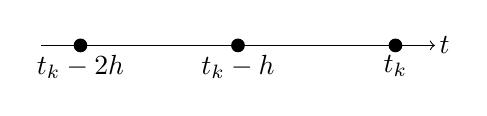
\begin{tikzpicture}[scale=2, domain=-0.5:2.5]
	\draw[->] (-.25,0) -- (2.25,0) node[pos=1.025] {$t$};
	\draw[fill=black] (0,0) circle [radius=0.04] node[below] {$t_k - 2h$};
	\draw[fill=black] (1,0) circle [radius=0.04] node[below] {$t_k - h$};
	\draw[fill=black] (2,0) circle [radius=0.04] node[below] {$t_k$};
	\end{tikzpicture}
	\end{center}

	For the Lagrange polynomials in the points $t_k$, $t_k -h$ resp. $t_k -2h$ we have
	\begin{gather*}
		L_0 (t) = \tfrac{t-(t_k-h)(t-t_k)}{2h^2}, \,
		L_1 (t) = \tfrac{(t-t_k)(t-t_kj-2h)}{h^2} \, \text{resp.} \,
		L_2 (t) =  \tfrac{(t-t_k+2h)(t-t_k+h)}{2h^2}.
	\end{gather*}

	As announced, we assume that the interpolation polynomial fulfilles the IVP in 
	the point $t_k$, i.e. there holds $f_k := f(t_k, y(t_k)) = y'(t_k) = \sum_{j=1} ^s 
		y_{k-j} L_{k-j} ' (t)$. The product rule and evaluation at $t=t_k$ yields

	\begin{gather*}
		L_0 '(t) = \tfrac{2t-2t_k+h}{2h^2} = \tfrac{1}{2h}, \,
		L_1 '(t) = -\tfrac{2t -2t_k + 2h}{h^2} = -\tfrac{2}{h}  \, \text{and} \,
		L_2 '(t) = \tfrac{2t-2t_k + 3h}{2h^2} = \tfrac{3}{2h}. 
	\end{gather*}

	Then, we obtain 
	\begin{gather*}
		f_k = \tfrac{1}{2h} y_{k-2} - \tfrac{2}{h}y_{k-1} + \tfrac{3}{2h} y_k.
	\end{gather*}
	Multiplication with $\tfrac{2}{3h}$ yields the scheme
	\begin{gather*}
		y_k - \tfrac{4}{3} y_{k-1} + 3y_{k-2} = \tfrac{2}{3h} f_k.
	\end{gather*}

%%% Local Variables: 
%%% mode: latex
%%% TeX-master: "notes"
%%% End: 
